\documentclass[a4paper,10pt]{article}
%-----------------------------------------------------------
\usepackage[top=0.75in, bottom=0.75in, left=0.55in, right=0.85in]{geometry}
\usepackage{graphicx}
\usepackage{url}
\usepackage{palatino}
\usepackage{tabularx}
\fontfamily{SansSerif}
\selectfont

\usepackage[T1]{fontenc}
\usepackage
%[ansinew]
[utf8]
{inputenc}

\usepackage{color}
\definecolor{mygrey}{gray}{0.75}
\textheight=9.75in
\raggedbottom

\setlength{\tabcolsep}{0in}
\newcommand{\isep}{-2 pt}
\newcommand{\lsep}{-0.5cm}
\newcommand{\psep}{-0.6cm}
\renewcommand{\labelitemii}{$\circ$}

\pagestyle{empty}
%-----------------------------------------------------------
%Custom commands
\newcommand{\resitem}[1]{\item #1 \vspace{-2pt}}
\newcommand{\resheading}[1]{{\small \colorbox{mygrey}{\begin{minipage}{0.975\textwidth}{\textbf{#1 \vphantom{p\^{E}}}}\end{minipage}}}}
\newcommand{\ressubheading}[3]{
\begin{tabular*}{6.62in}{l @{\extracolsep{\fill}} r}
	\textsc{{\textbf{#1}}} & \textsc{\textit{[#2]}} \\
\end{tabular*}\vspace{-8pt}}
%-----------------------------------------------------------

\begin{document}
\hspace{0.5cm}\\[-0.2cm]

\centering
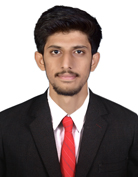
\includegraphics[]{35x45.jpg}\\
\underline{\textbf{ ABHISHEK PATHAK}} \\
\indent 28, Patel Park Society, 
\indent near old RTO Warasiya,  \\
\indent Vadodara (Gujarat, INDIA) - 390006\\
\indent \textbf{Email-id} : pathakabhi897@gmail.com \\
\indent Mobile No.: \textbf{7778016301} \\

\resheading{\textbf{ CAREER OBJECTIVE} }\\[\lsep]
\begin{itemize}
    \item Aspire to obtain the position of an engineer in a respectable firm where I can fully utilize my talent, knowledge, proficiency and excellent communication and interpersonal skills for the benefit of firm.
\end{itemize}\\

\resheading{\textbf{ACADEMIC DETAILS} }  \\
\hspace{.2 cm}
\begin{itemize}
    \item \noindent Pursuing Bachelor of Engineering (BE) in 8th semester from Mechanical Engineering.
\end{itemize}

%\begin{table}[ht!]
%\begin{center}
\indent \begin{tabular}{ l @{\hskip 0.15in} l @{\hskip 0.15in} l @{\hskip 0.15in} l @{\hskip 0.15in} l @{\hskip 0.15in} l }
\hline
\textbf{Sr. No.} & \textbf{Examination} & \textbf{University} & \textbf{Institute} & \textbf{Year} & \textbf{CPI/\%} \\
\hline
1. & SSC & GSEB & Lal Bahadur Sashtri Vidhyalay & 2012 & 79 \\
2. & Diploma & Gujarat Technological University & Butler Polytechnic & 2015 & 7.85\\
3. & BE cont.. & Gujarat Technological University & Vadodara Institute of Engineering & 2018 & 7.2\\
\hline
\end{tabular}
%\end{center}
%\end{table}
\\ \\

\hspace{1 cm}
\resheading{\textbf{PROJECTS} }\\[\lsep]
\begin{itemize}

\item \underline {\textbf{Automatic Tin Cutting Machine 
 (Diploma Project)}} \\ \\[-0.6cm] 
	\begin{itemize}\itemsep \isep
	\item \textbf{Duration : 5-6th Semester}  
	\item This machine is use to cut the Tin material by using Pneumatic Double Acting Cylinder.
.
	\item The Cylinder is operated by compressed Air.

	\end{itemize}
	
	\item \underline{ \textbf{Automatic Board Rubbing Machine (BE: Design Engineering Project)} } \\
	\begin{itemize}
	    \item \textbf{Duration : 5-6th Semester}
	    \item This machine is automatically rub the board by using camera and sensor.
	    \item It reduce the time and human effort during lecture.
	\end{itemize}
	
\item \underline{\textbf{Automatic Stirrup Making Machine
 (BE - Final Year Project) }} \\
	\begin{itemize}\itemsep \isep
	\item \textbf{Duration : 7-8th Semester} 
	\item This Machine is use to make the stirrups by bending rods of require shape and size as per the requirement of beams and columns.
	\item The main objective of this project is to eliminate the manual operation of stirrup making and converting it to automation.
	\end{itemize}
\end{itemize}

\resheading{\textbf{TRAINING / INTERNSHIP} }\\[\lsep]
\begin{itemize}
    \item \noindent Attended an Industrial training \& internship at   \textbf{ Mitsubishi Electric India Privet Limited } in October  2017.\\
        \begin{itemize}
        \item Successfully completed the training course in the following..
        \item PLC
        \item HMI
        \item VFD 
        \item Servo Motor
        \end{itemize}
    \item \noindent Attended 10 days Industrial Training at \textbf{ Varahi Engineering} on May 2017.
    \item \noindent Attended the Training Program on Basics of Pneumatics with \textbf{ Janatics Animation Software for Pneumatic } in July 2016.
        \begin{itemize}
        \item Courses are..
        \item Circuit designing of Pneumatic valves 
        \item Different Pneumatic Component like cylinders, pressure gauge, compressor, solenoid Valves of various types and etc..
        \end{itemize}
    \item \noindent Attended the workshop on Introduction to \textbf{CAM / CREO 2.0} at \textbf{ Zillion Technologies } in February 2015. 
\end{itemize}


\resheading{\textbf{FIELDS OF INTEREST} }\\[\lsep]
\begin{itemize}
\item \noindent Production
\item \noindent Pneumatic system
\item \noindent Mathematics
\item \noindent Aeronautical engineering
\item \noindent IC engines 
\item \noindent R \& D of new mechanisms   \end{itemize}

\resheading{\textbf{TECHNICAL SKILLS} }\\[\lsep]
\begin{itemize}
\item \noindent Good knowledge Of Hydraulics \& Pneumatic system
\item \noindent Conventional machines operation like (Lathe, Drilling, Milling, Cutting, etc..)   
\item \noindent 3D printer operating 
\item \noindent Critical Problem Solver 
\item \noindent Research \& development of innovative Mechanism
\end{itemize}


\resheading{\textbf{SOFT SKILL} }\\[\lsep]
\begin{itemize}
\item \noindent Positive work attitude with dedication 
\item\noindent Self motivated 
\item\noindent Ability to learn new things quickly
\item\noindent Team work
\item\noindent Social interaction
\item\noindent Hardworking
\end{itemize}

\resheading{\textbf{HOBBIES} }\\[\lsep]
\begin{itemize}
\item \noindent Learn new things
\item \noindent Sports like (Cricket, Volleyball, Table Tennis)
\item \noindent To watch Discovery channel 
\item \noindent To listen Soft music  
\end{itemize} 




\resheading{\textbf{CO-CURRICULAR ACTIVITIES}  }\\ [\isep]
\begin{itemize}
    \item \underline{\textbf{YEAR 2018}}
    \begin{itemize}
    
    \item  Participation in National competition \textbf{ Mitsubishi Electric Cup 2018 } held at Nirma University, Ahmedabad on February 2018.
    \item \noindent Participation in \textbf{National Robocon 2018} held at Pune Balewadi Stadium,in March 2018.
    \item \noindent Certificate on Participation in \textbf{ Tech Eureka} in the State leval Technical festival Organize by \textbf{ GCET } Vallabh Vidyanagar, Gujarat, on April 2018.
    \item \noindent  Certificate on participation in the Regional Final of the \textbf{ e-Yantra Ideas Compitition (eYIC 2018) } held at \textbf{  (IIT RAM) } Ahmedabad, on February 2018.
    \end{itemize}
    
    \item \underline {\textbf{YEAR 2017}}
    \begin{itemize}
    
    \item \noindent Participation in National level competition \textbf{ World Robotics Olympiad }(Advance Robotic Category) held at Delhi in October 2017. 
    \item \noindent Participation in \textbf{National Robocon 2017} held at Pune Balewadi Stadium,in March 2017.
    \item \noindent Certificate on Participation in \textbf{ Fast N' Furious } held at \textbf{ (VJTI) } Matunga, Mumbai  on December 2017. 
    \item \noindent Certificate on Participation in \textbf{ Full Throttle } National level Techfest held at \textbf{IIT BOMBAY } Powai, Mumbai on December 2017.
    \item \noindent Certificate on Participation in \textbf{ Fast N' Furious (Robotics) }  in National level Technical Symposium Prakash 2017 held at \textbf{ SVIT }, Vadodara  on February 2017.
    \item \noindent Certificate on Participation in \textbf{ Working Model } Illuminati 2017  held at \textbf{ITM Universe } Vadodara  , Gujarat on February 2017.
    \item \noindent Certificate on Participation in \textbf{ Burnout } FootprintT 2017  held at \textbf{MS University } Vadodara, Gujarat on February 2017.
    \end{itemize}
    
    \item \underline{\textbf{YEAR 2016}}
    \begin{itemize}
    
    \item \noindent Participation in \textbf{ Robotics Competition }(Line follower Robot) on the theme \textbf{ Make In India } under the banner of \textbf{ISTE}(Indian Society For Technical Education) Gujarat selection held at Rajkot , in October 2016.
    \item \noindent Participation in \textbf{National Robocon 2016} held at Pune Balewadi Stadium,in March 2016.
    \item \noindent Certificate on Participation in \textbf{ Full Throttle } National level Techfest held at \textbf{IIT Bombay } Powai, Mumbai on December 2016.
    \item \noindent Certificate on Participation in \textbf{ Robotics } Competition on the theam \textbf{Make In India} under the banner of \textbf{ISTE}(Indian Society For Technical Education) Gujarat selection held at Rajkot, in October 2016.
    \item \noindent Certificate on Participation in \textbf{ Agro Quiz } Competition on the theam \textbf{Make In India} under the banner of \textbf{ISTE}(Indian Society For Technical Education) Gujarat selection held at Rajkot, in October 2016.
    \end{itemize}
    
    \item \underline{ \textbf{YEAR 2014}}
    \begin{itemize}
    
    
    \item \noindent Certificate on Participation in \textbf{ Wanderllar} event in GTU ZONAL TECHFEST held at \textbf{Babaria Institute Of Technology (BITS) } Vadodara, Gujarat on March 2014.
    \end{itemize}
    
\end{itemize}

\resheading{\textbf{ACHIEVEMENTS}  }\\ [\isep]

\begin{itemize}
   
   \item \underline {\textbf{YEAR 2018 }}
   \begin{itemize}
   
   \item \noindent Winner of National Level Competition \textbf{ e-Yantra Ideas Competition (eYIC-2018) }.\\
   \item Also awarded with \textbf{ Best Demonstration \& Participation Award } and Best Judge Choice award at IIT, Bombay in April 2018.
   \item \noindent Achieved 7th position in all over India for the National competition \textbf{ Mitsubishi Electric Cup 2018} held at \textbf{ Nirma University}, Ahmedabad on February 2018.
   \item \noindent Achieved 2nd Rank in \textbf{Machine Mania} in VIROTSAV held at Vadodara Institute Of Engineering on February 2018.
   \end{itemize}
   \item \underline {\textbf{YEAR 2017}}
   \begin{itemize}
   
   \item \noindent Winner in National level Competition \textbf{ World Robotic Olympiad} held at Delhi in October 2017.
   \item \noindent 2nd Runner up in \textbf{ National Robocon 2017} held at Balewadi Stadium Pune, Maharastra on February 2017.
   \end{itemize}
   
   \item \underline {\textbf{YEAR 2016}}
   \begin{itemize}
   
   \item \noindent Winner in \textbf{ Robotics Competition (Line Follower Robot) } on the theam \textbf{Make in India} under the banner of \textbf{ISTE}(Indian Society For Technical Education) Gujarat selection held at Rajkot, in October 2016. 
   \item \noindent Best Design Award in \textbf{ International Robocon 2016} held at \textbf{BANGKOK, THAILAND } in August 2016.
   \item \noindent Winner in \textbf{ National Robocon 2016} held at Balewadi stadium Pune, Maharastra on February 2016.
   \end{itemize}
\end{itemize}

 \resheading{\textbf{PERSONAL DETAIL}  }\\ [\isep]
  \begin{itemize}
      \item \textbf{Father's Name} : Sanjay Ramakant Pathak
      \item \textbf {Mother's Name} : Pallavi Sanjay Pathak
      \item \textbf {Gender}           : Male
      \item \textbf {Date Of Birth} : 8 April 1997 
      \item \textbf {Nationality}   : Indian
      \item \textbf {Languages Known}: English, Hindi, Gujarati
      \item \textbf {Mothertongue }  : Marathi
      \item \textbf {Marital Status}: Unmarried 
  \end{itemize}
  \resheading{\textbf{REFERENCES}  }\\ [\isep]
   \begin{enumerate}
       \item \textbf{Dr. Jayeshkumar S Patel}\\
       \ principal\\
       \ Vadodara Institute Of Engineering \\
       \ Vadodara \\
       \ Contact : 0265-3915900-1-2-3-4 \\
       \ Email : vierorgin@yahoo.com \\
       
       \item \textbf{Prof. Satish Bhati} \\
       \ Assistant professor \\
       \ Vadodara Institute of Engineering \\
       \ Vadodara \\
       \ Mobile : +919909959321 \\
       \ Email : bhatisatish4045@gmail.com \\
       
       \item \textbf{Prof. Vimal B Patel} \\
       \ GTU Coordinator \\
       \ Vadodara Institute of Engineering \\
       \ Vadodara \\
       \ Mobile : +919624560842 \\
       \ Email : vml310@gmail.com\\
   \end{enumerate}
 \resheading{\textbf{DECLARATION}  }\\ [\isep] 
 \begin{itemize}
     \item \noindent I hereby declare that the above mentioned information is true to the best of my knowledge.
 \end{itemize}
 
 \hspace{ 7.0 cm}
 \begin{itemize}
     
 \end{itemize}
 
 \raggedright{Date : 19 April 2018}\\ \raggedleft{Abhishek Pathak}
\end{document}